\documentclass[parskip=half]{scrartcl}
\usepackage{amsmath}
\usepackage[T1]{fontenc}

\usepackage{graphicx}

\usepackage{natbib}

\bibliographystyle{agufull08}
\newcommand{\changefont}[3]{\fontfamily{#1} \fontseries{#2} \fontshape{#3} \selectfont}

%% commands to facilitate units and temperature
\newcommand{\unit}[1]{\ensuremath{\,\mathrm{#1}}}
\newcommand{\s}[1]{\ensuremath{\,\mathrm{#1}}}
\newcommand{\cels}[1]{\ensuremath{#1^{\circ}\,\mathrm{C}}}


% ---------------------------------------------------------------------------------------
% definition of header and footer
% ---------------------------------------------------------------------------------------

\usepackage[automark,headsepline,footsepline]{scrpage2}
\clearscrheadings	
\ihead{Dynamics of glaciers}
\ohead{McCarthy Summer School 2014}
\cfoot{\pagemark}
\setkomafont{pagehead}{\normalfont}	
\setkomafont{pagenumber}{\normalfont\rmfamily}




% ---------------------------------------------------------------------------------------
% Koma-Script - Settings
% ---------------------------------------------------------------------------------------
\addtokomafont{caption}{\small}
\setkomafont{captionlabel}{\sffamily\bfseries}
% \setkomafont{caption}{\sffamily}
\setcapindent{1em}

\pagestyle{scrheadings}


\begin{document}

\vspace{-5em}

\title{Dynamics of Glaciers \\[.2em]
\rule[1em]{\textwidth}{2pt}
\LARGE{\sf Exercise}
}
\date{}

\vspace{-5em}

\maketitle


\vspace{-5em}

\section{Flow speeds}

Will and Carl are two grad students in glaciology who are really excited about their first opportunity to do field work on Kennicott Glacier, Alaska. Arriving in the town of McCarthy, their spirits are slightly dampened by heavy fog that makes it impossible to see Root Glacier from their tent. They decide to get started by going through the scribbles left by former grad student Tim. In Tim's field book they discover a sketch of Kennicott and Root Glacier (see Figure~\ref{fig:map}) and a note that the average ice thickness is 900\,m. Later that evening, at the bar,  Will and Carl make a bet who can better guess the surface speed of Kennicott Glacier between Hidden Creek Lake and Donahue Falls Lake. Recalling the glacier dynamics course they took the previous semester, Will assumes that Root Glacier can be approximated by an inclined parallel-sided slab and that half of the surface motion is due to basal sliding. Carl, on the other hand, opts for a cylindrical channel. 

\paragraph{Question} During the second day, Will and Carl find a hard disk with GPS velocities from GPS station 3. They're surprised to discover that the average surface speed is around 0.5 meters per day. Who made the better guess and won the beer at the bar that night?
\\[1em]
Hint: assume a rate factor $A=2.4\cdot 10^{-24}\,\textrm{s}^{-1}\,\textrm{Pa}^{-3}$


\begin{figure}
  \centering
   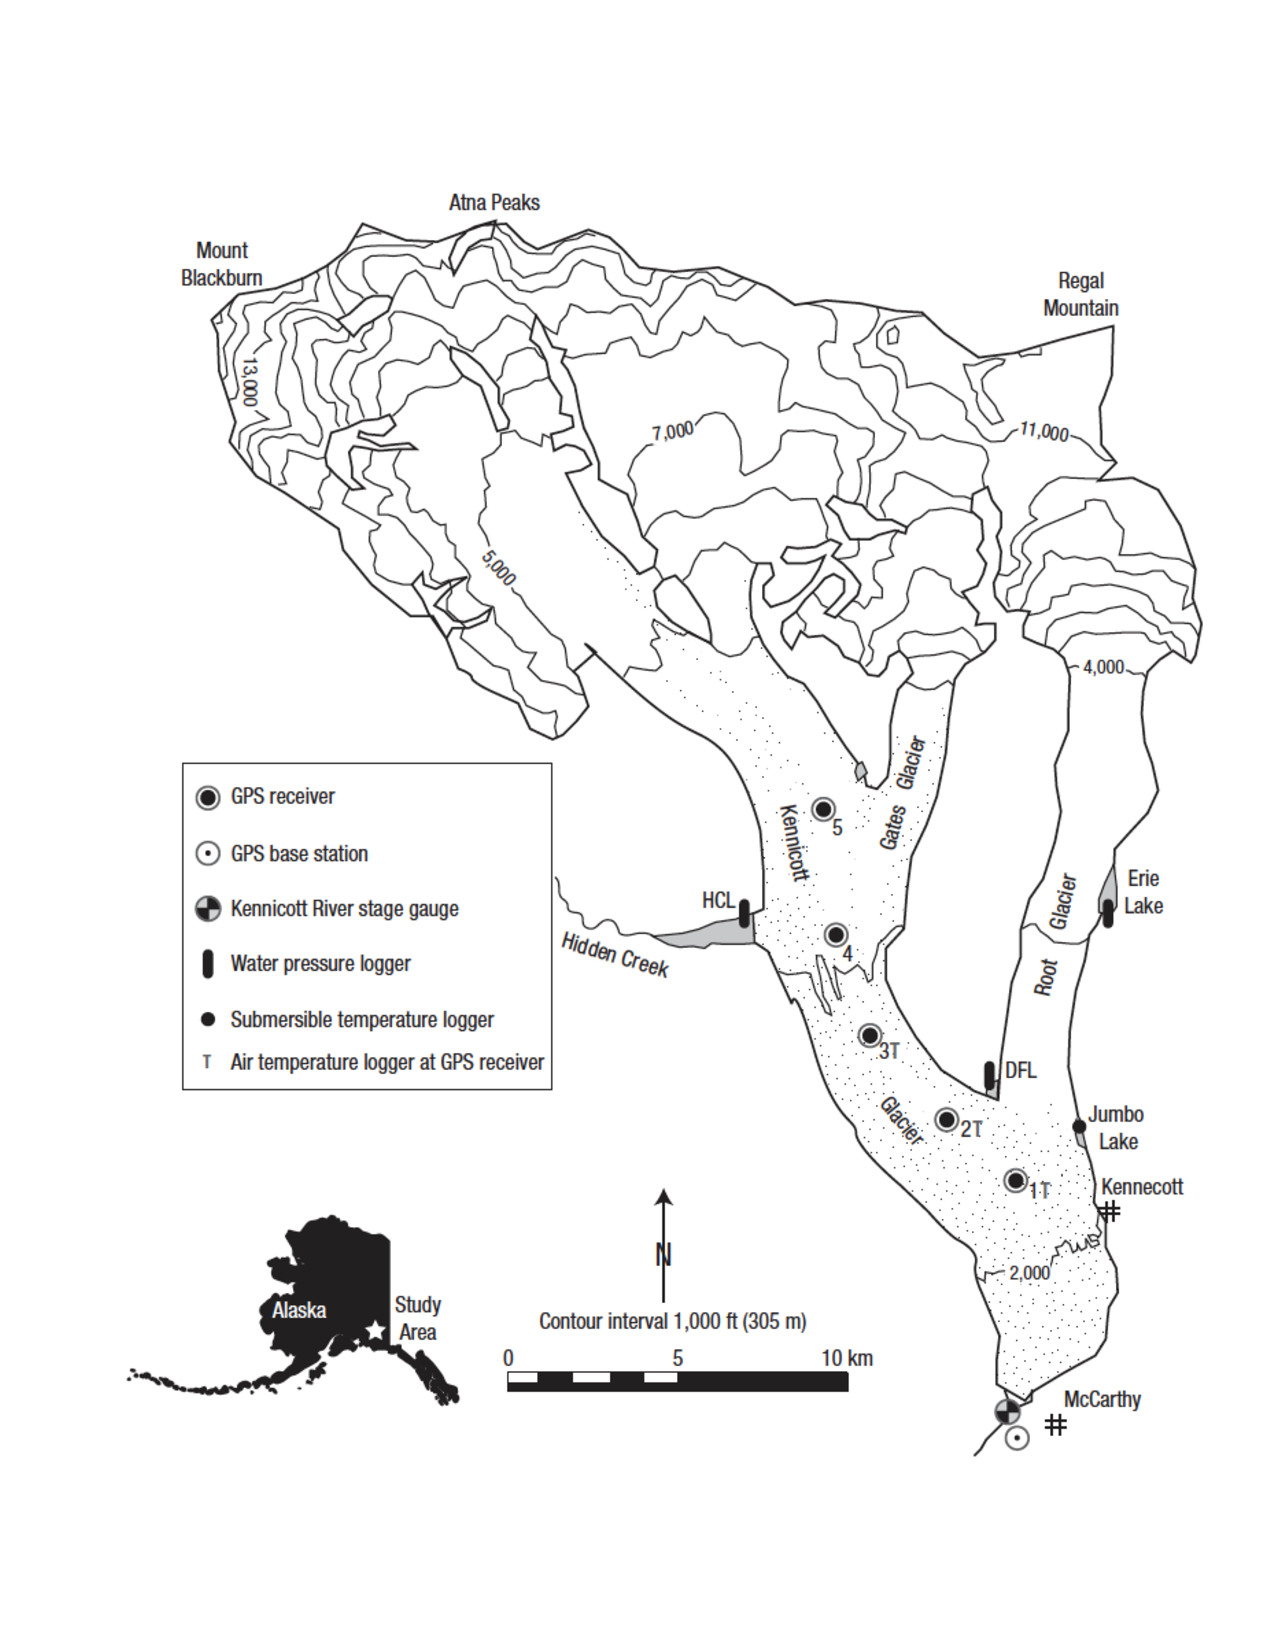
\includegraphics[width=14cm]{figures/barth-map} 
   \label{fig:map}
   \caption{Map from \cite{Bartholomaus2008}}
\end{figure}

\section{Mass flux}

Fortunately the weather clears up and Will and Carl spend the better part of a week collecting additional ice thickness measurments with their ground penetrating radar. Since it's late summer, they have to carry the radar around by hand, a really laborious task. They conclude that collecting radar data is easier in spring when you can ski or snowmachine, simply draggin the radar behind. Nonetheless, with an ice thickness profile across the glacier, passing through GPS site 3 and the velocity readings from the same GPS, Will and Carl intend to calculate the mass flux through site 3. They know that the mass flux $Q$ is given by

\begin{equation}
Q = \bar v H = \int \limits_0^H v\, \mathrm{d}z,
\end{equation}
where $\bar v$ is the vertically-averaged horizontal flow speed and $H$ is the ice thickness. Will and Carl only know the surface speed but not the depth distribution. Will realizes that in the case of plug flow (i.e. all horizontal motion is due to basal sliding) the vertically-averaged velocity is equal to the surface velocity. Carl then suggests that in the case of no basal sliding (i.e. vertical shearing only), the vertically-averaged horizontal velocity should be lower than for plug flow.

\paragraph{Question} Is Carl right, and if so, by how much?

\section{Melting temperature depression}

What is the pressure melting temperature at the base of Gornergletscher (Fig.~9)? What does the Clausius-Clapeyron relation indicate in terms of air-saturation of the meltwater? The pressure $p$ is the sum of the hydrostatic pressure and the atmospheric pressure, $p = \rho g H + p_{\text{atm}}$. Assume $p_{\text{atm}} = 75\,\text{kPa}$.

\section{Lake Vostok}

\begin{enumerate}
\item Describe 2 different ways how heat can be moved through a polar ice sheet.
\item What is the P\'eclet Number, and how is it useful?
\item The coldest temperature ever recorded is -\cels{89} at Vostok in East Antarctica (in July 1983). The mean annual temperature is -\cels{55}. However, deep under the ice is lake Vostok, a lake of the size of lake Ontario. Calculate the minimum geothermal flux needed for a lake to form. Possibly relevant quantities:
  \begin{itemize}
  \item Surface elevation $3488\,\text{m}$
  \item Ice thickness $3300\,\text{m}$
  \item Snow accumulation rate $2\,\text{cm}\,\text{a}^{-1}$ (water equivalent)
  \item A reasonable average thermal conductivity for the cold temperatures of the East Antarctic Ice Sheet is $k = 2.5\,\text{W}\,\text{m}^{−1}\,\text{K}^{−1}$.
  \end{itemize}
\end{enumerate}
\bibliography{thermobib}
\end{document}